\documentclass[a4paper]{article}
\usepackage[utf8]{inputenc}
\usepackage[english]{babel}
\selectlanguage{english}
\usepackage{amsthm}
\usepackage{graphicx}
\usepackage{float}
\usepackage{subfig}
\usepackage{multirow}

\author{Bas Vlaszaty \\ 5783445 \\ Bas.Vlaszaty@student.uva.nl \\ \& 
  \\ Joost Hekman \\ 5887232 \\ Joost.Hekman@student.uva.nl}

\title{Small-world networks}

\theoremstyle{definition}
\newtheorem*{swn-def}{Definition}

\begin{document}

\maketitle

\begin{center}
  \begin{figure}[H]
    \centering
    
\includegraphics[scale=0.7]{barabas.jpg}
    \caption{Professor Barabas}
    \label{fig:barabas}
  \end{figure}
\end{center}

\newpage
\tableofcontents

\newpage
\section{Introduction}
Here we will introduce the assignment and how we planned our elaboration.\\

The assignment consisted of two main parts. The first part wanted us to
either create or find an algorithm that could build a number of small-world
networks, ranged from completely random to completely regular. Then we were
charged with finding interesting variables that we could use to compare each
of these networks. Suggestions were clustering, diameter or robustness but
we were free to find other, maybe even better data that we can use in our
examination of small-world networks.\\

The second part wanted us to take one of these small-world networks and
apply a SIR model to it. SIR stands for Susceptible, Infected and
Recovered/Resistent and its widely used for modelling infectious diseases to
predict the spreading of the disease. We specifically needed to examine the
effect of vacination at the beginning of a small-world network by labelling
some random number of nodes at the beginning with R as them being
resistent.\\

Our planning was as followed: we first start reading about small-world
networks, then we decided which of the small-networks was best to compare to
each other. Next thing we devided the algorithms in two so that we each
could start working on other algorithms independently. This allows us to
work faster and dive deeper into the algortims then would be normally 
possible. After doing the research, we would implement the methods we each
had chosen, then we would compare them. Next thing would be applying an
algorithm to the SIR model, which we do together. Finally we would be putting
our results into a report and hand it in together with our source code.

\newpage
\section{Small-world network}
This section will explain what Small-world networks are and give some
requirements on when a network is considered to be a small-world network.\\

In a small-world network, nodes that represent it are mostly not everybody's
neighbor but each node can be reached from every other node by taking a
relatively small number of steps inside this graph. Moreover, this number is
actually defined in relation to the number of nodes $N$ present in the
graph. The definition is as follows:

\begin{swn-def}
$L \propto$ log $N$
\end{swn-def}

Certain kinds of small-world networks exhit a behaviour similar to random
graphs. This means they have a small average path length, which means how 
many steps you have to take to get from any randomly chosen node to another.
Also, the so called clustering coefficient which describes how nodes group
together is very low on most random networks, but not necesarilly so on the
small-world networks. For instance, the network algoritm from Duncan Watts
and Steven Strogatz has a relatively high clustering coefficient compared
to pure random networks. More on this network follows below.\\

Small-world networks tends to form so-called sub-networks of nodes which
have connections to at least two nodes within them. This relates to the
small average path length of these networks because you can travel faster
trough these sub-networks then you can when you are only connected to one
big network.\\

Some small-world networks exhibit more of a behaviour know as a scale-free
network, which means they form so called hubs which are node with a very
high degree of edges to other nodes. In these networks there are no ring
structures so the clustering is absent. This mean they can form networks
with a small average path length with fewer edges than a network with a high
clustering coefficient which uses sub-networks with cicles.\\

\newpage
\subsection{Watts-Strogatz}
Here we provide some explenation about the Watts-Strogatz method of building
a small-world network.\\

Watts-Strogatz is an algorithm to create a random graph with small world properties. It has high clustering and short average path length. The algorithm was proposed in 1998.
The algorithm takes 3 variables:\\

\begin{enumerate}
 \item \texttt{N}: The number of nodes in the graph
 \item \texttt{K}: The mean degree of the nodes. 
 \item \texttt{b}: The probability of a connection to be rewired. Can also be seen as the degree of randomness. 
\end{enumerate}

The Watts-Strogatz algorithm consists of two steps:\\

\begin{itemize}
  \item \emph{Constuct}\\
    First we create a ring of nodes. Each node is connected to its K neigbours on each side, so for K=2, node 6 would be connected to 4, 5, 7 and 8.
  \item \emph{Rewiring}\\
    Once the ring has been created, we are going to rewire some of its connections. To do this we will loop through all the connections of the node, and with probability b rewire them to connect to a random different target. It is not allowed to connect to self, or to duplicate a connection that already exists. As you can imagine a higher b means that we randomly rewire more connections, and the graph structure will diverge more and more from the ring it started out as. If we choose b very low, just a couple of connections will be rewired, and the structure will stay as it was for large parts. 
\end{itemize}

\newpage
\subsubsection{Graphs}
Here we plot some networks from different sizes that uses the Watts-Strogatz
method.\\
\begin{figure}[H]
  \centering
  \subfloat[N = 10]{
    \label{fig:random-graph10}
    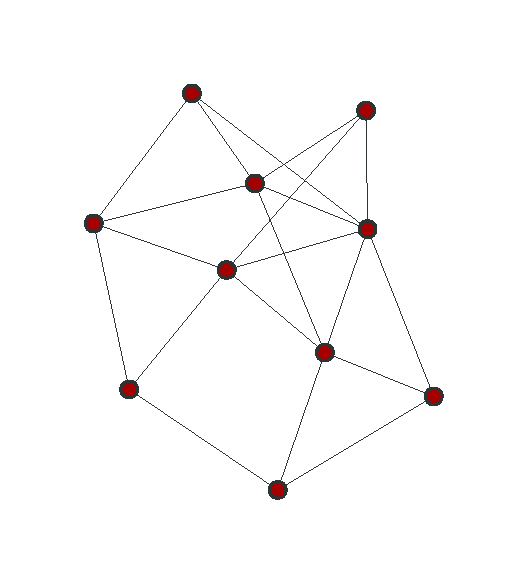
\includegraphics[width=0.4\textwidth]{../graphs/random10.pdf}
  }
  \hspace{1em}
  \subfloat[N = 100]{
    \label{fig:random-graph100}
    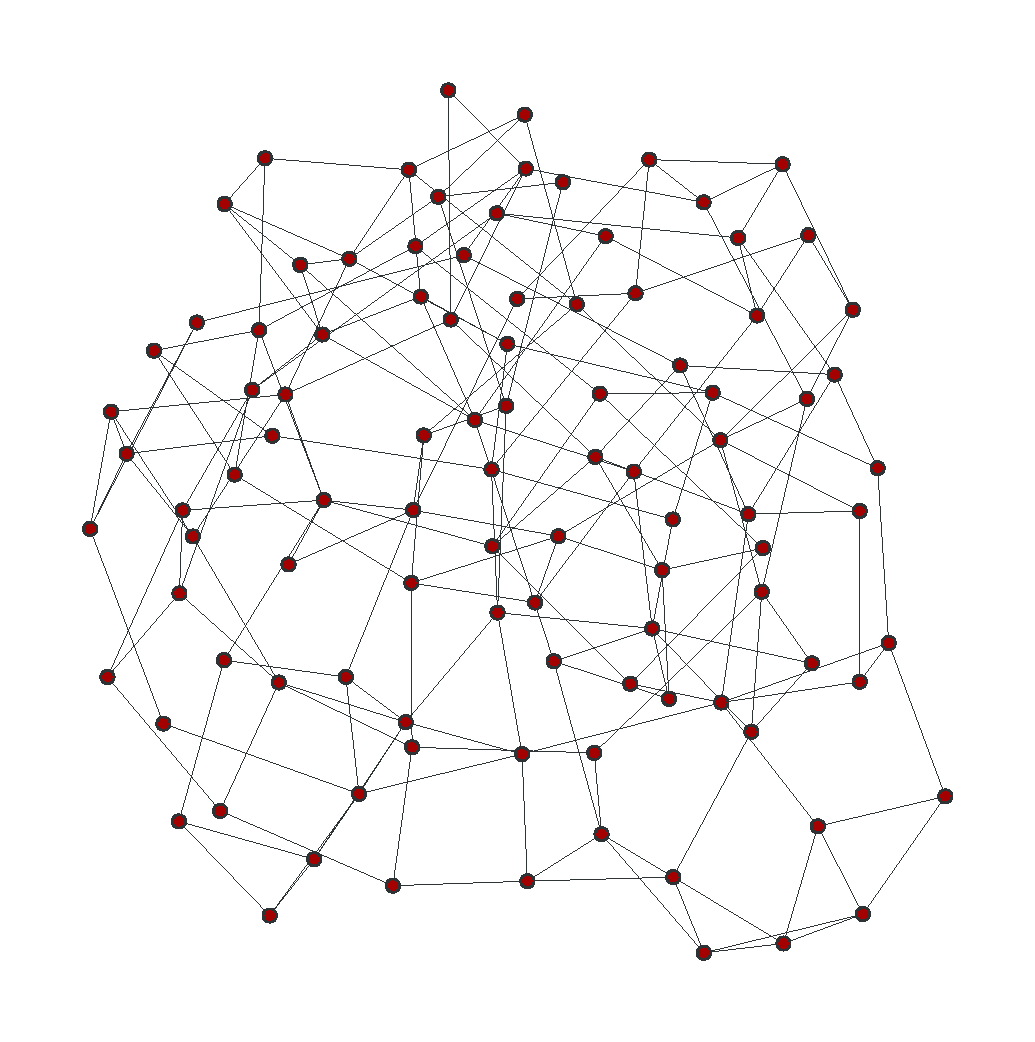
\includegraphics[width=0.4\textwidth]{../graphs/random100.pdf}
  }
  \hspace{1em}
  \subfloat[N = 1000]{
    \label{fig:random-graph1000}
    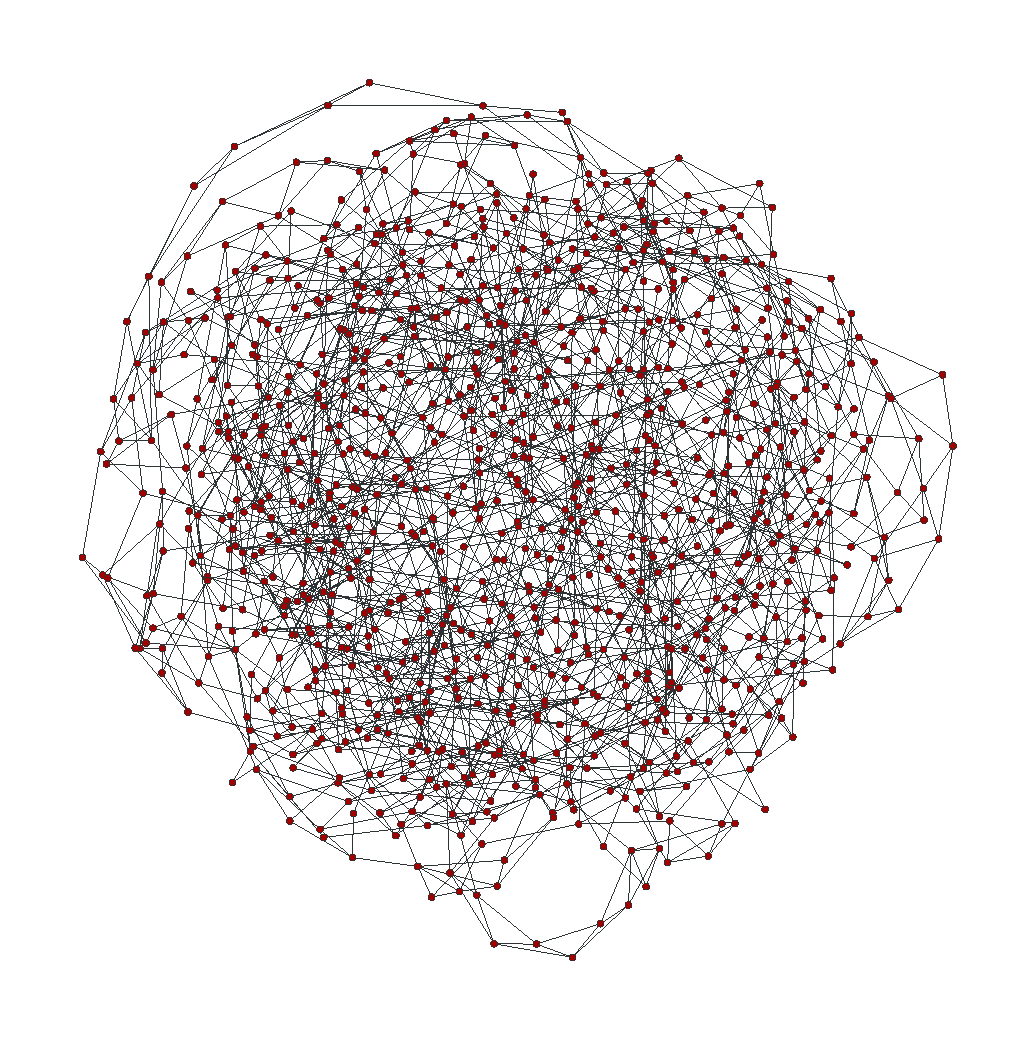
\includegraphics[width=0.4\textwidth]{../graphs/random1000.pdf}
  }
  \hspace{1em}
  \subfloat[N = 10000]{
    \label{fig:random-graph10000}
    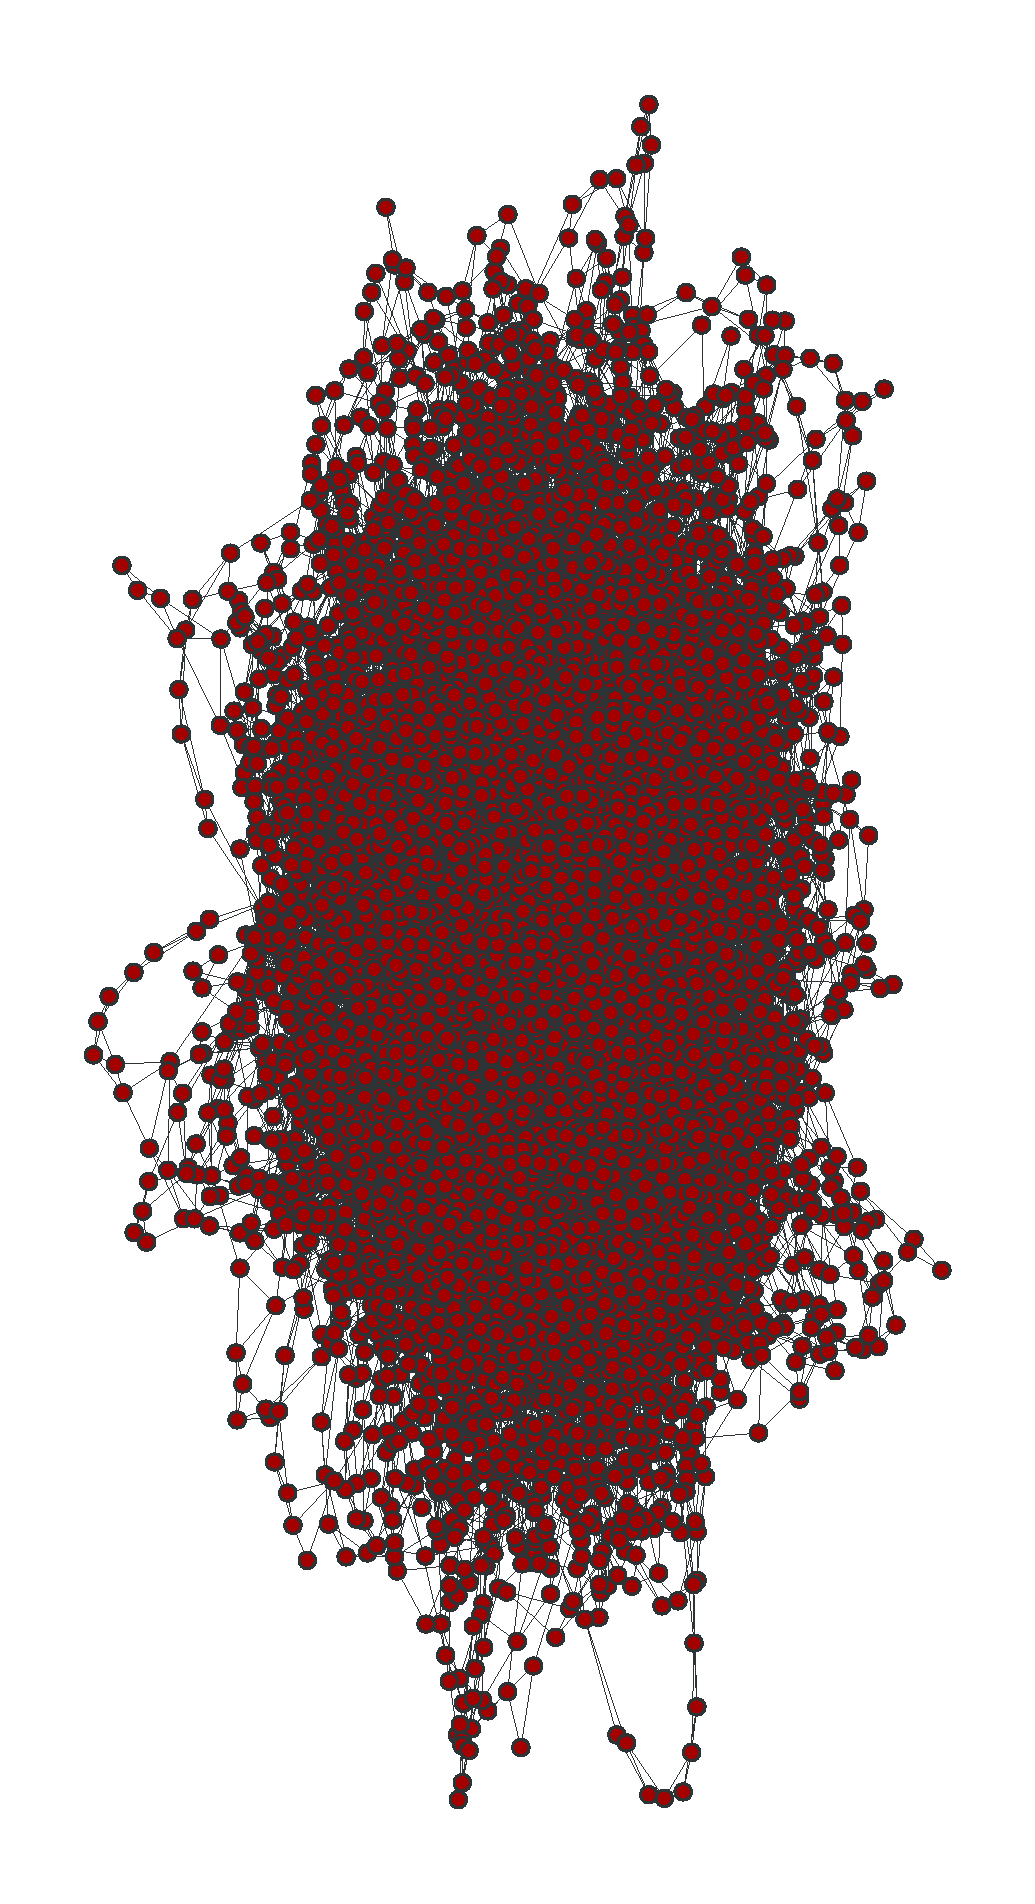
\includegraphics[width=0.4\textwidth]{../graphs/random10000.pdf}
  }
  \hspace{1em}
  \caption{Random ring networks with N nodes}
  \label{fig:random-graphs}
\end{figure}

\newpage
\subsubsection{Plots}
Here we display graphs about the total degree of the networks above.\\
\begin{figure}[H]
  \centering
  \subfloat[N = 10]{
    \label{fig:random-hist10}
    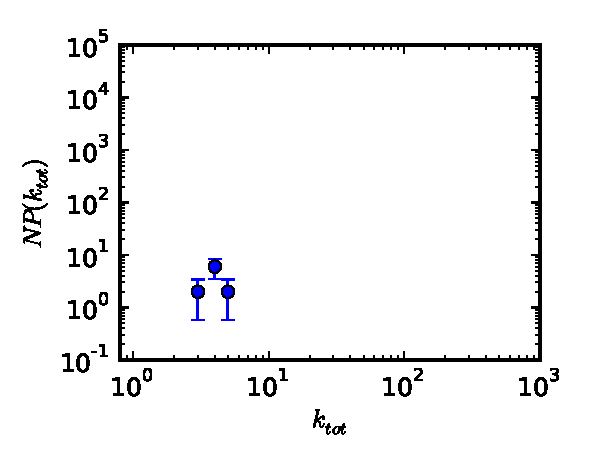
\includegraphics[width=0.4\textwidth]{../hist/random10.pdf}
  }
  \hspace{1em}
  \subfloat[N = 100]{
    \label{fig:random-hist100}
    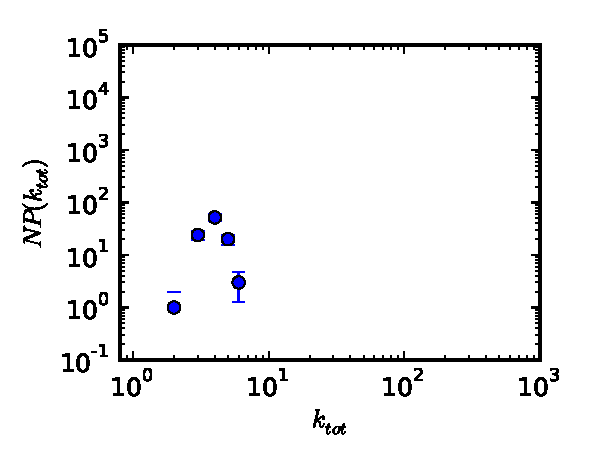
\includegraphics[width=0.4\textwidth]{../hist/random100.pdf}
  }
  \hspace{1em}
  \subfloat[N = 1000]{
    \label{fig:random-hist1000}
    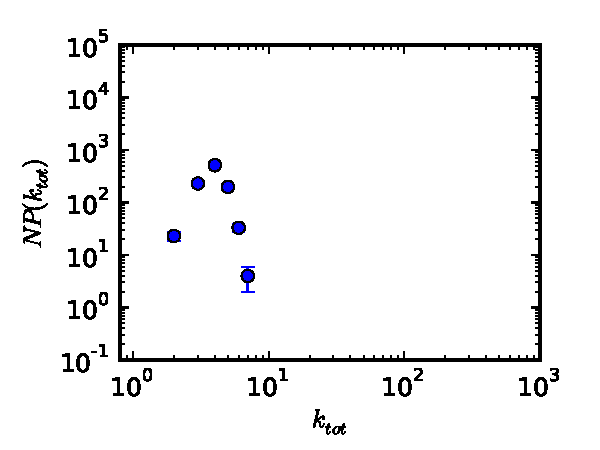
\includegraphics[width=0.4\textwidth]{../hist/random1000.pdf}
  }
  \hspace{1em}
  \subfloat[N = 10000]{
    \label{fig:random-hist10000}
    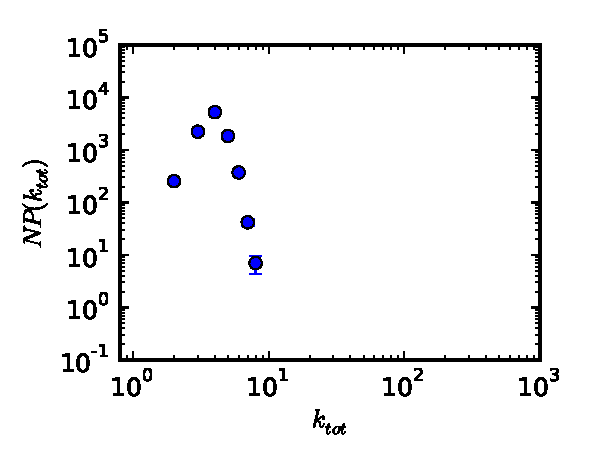
\includegraphics[width=0.4\textwidth]{../hist/random10000.pdf}
  }
  \hspace{1em}
  \caption{Total-degree histogram of random networks with N nodes}
  \label{fig:random-histograms}
\end{figure}

\newpage
\subsection{Barabasi}
Here we explain some information about the Barabasi small-world network
algorithm.\\

Albert Lazlo Barabasi discovered that there are some small-world networks
that not only form hubs but that their number of connections to other nodes
in the network had a so-called Power-law distribution. This means if you
plotted this distribution that it followed a certain asymptote formed like a
parabola.\\

As he progressed through his research, he came up with the name 'scale-free
networks', which had its application through out the biology, the internet
and many more.\\

The algoritm works like this:\\

If an node has more edges then other nodes, its propability of it getting
another edge would be higher. So, a node with three edges will have more
chance in getting its fourth edge then a node with two edges in getting its
third. This is called the Preferential attachment which can be applied even
to large en complex systems like the human population because in the old
times, wealthy and rich people get more income then the people who are less
fortuned.\\

\newpage
\subsubsection{Graphs}
Here we give some network of different sizes that uses the Barabasi
algorithm.\\
\begin{figure}[H]
  \centering
  \subfloat[N = 10]{
    \label{fig:scale-free-graph10}
    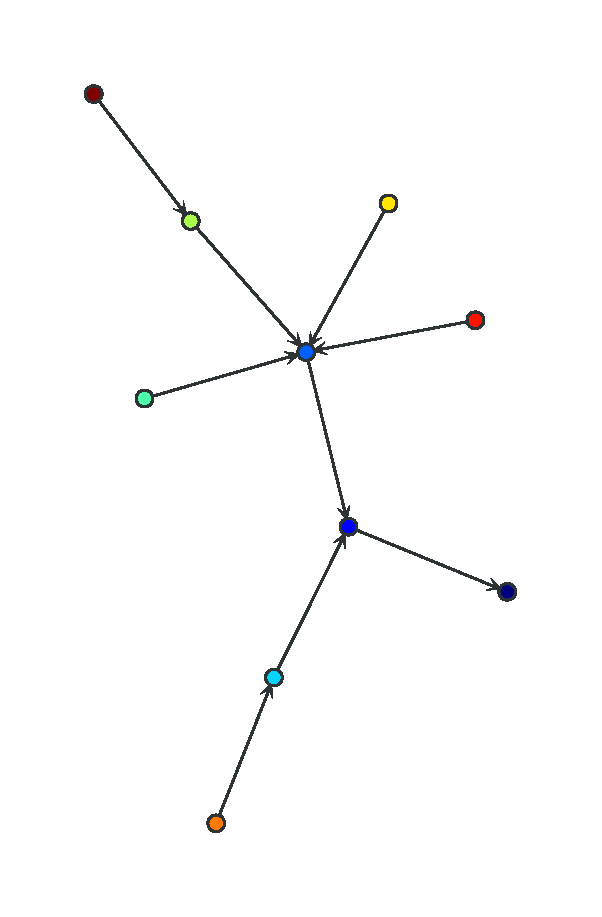
\includegraphics[width=0.4\textwidth]{../graphs/scale-free10.pdf}
  }
  \hspace{1em}
  \subfloat[N = 100]{
    \label{fig:scale-free-graph100}
    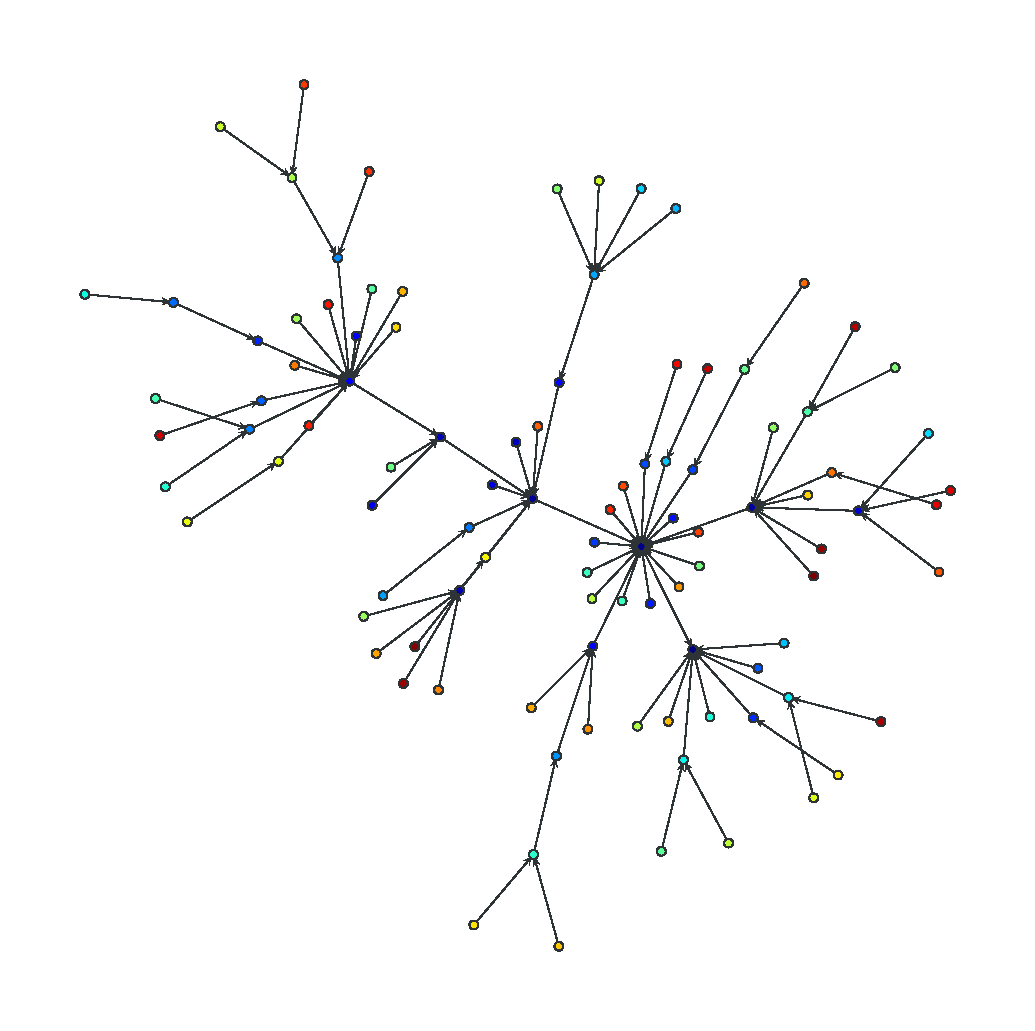
\includegraphics[width=0.4\textwidth]{../graphs/scale-free100.pdf}
  }
  \hspace{1em}
  \subfloat[N = 1000]{
    \label{fig:scale-free-graph1000}
    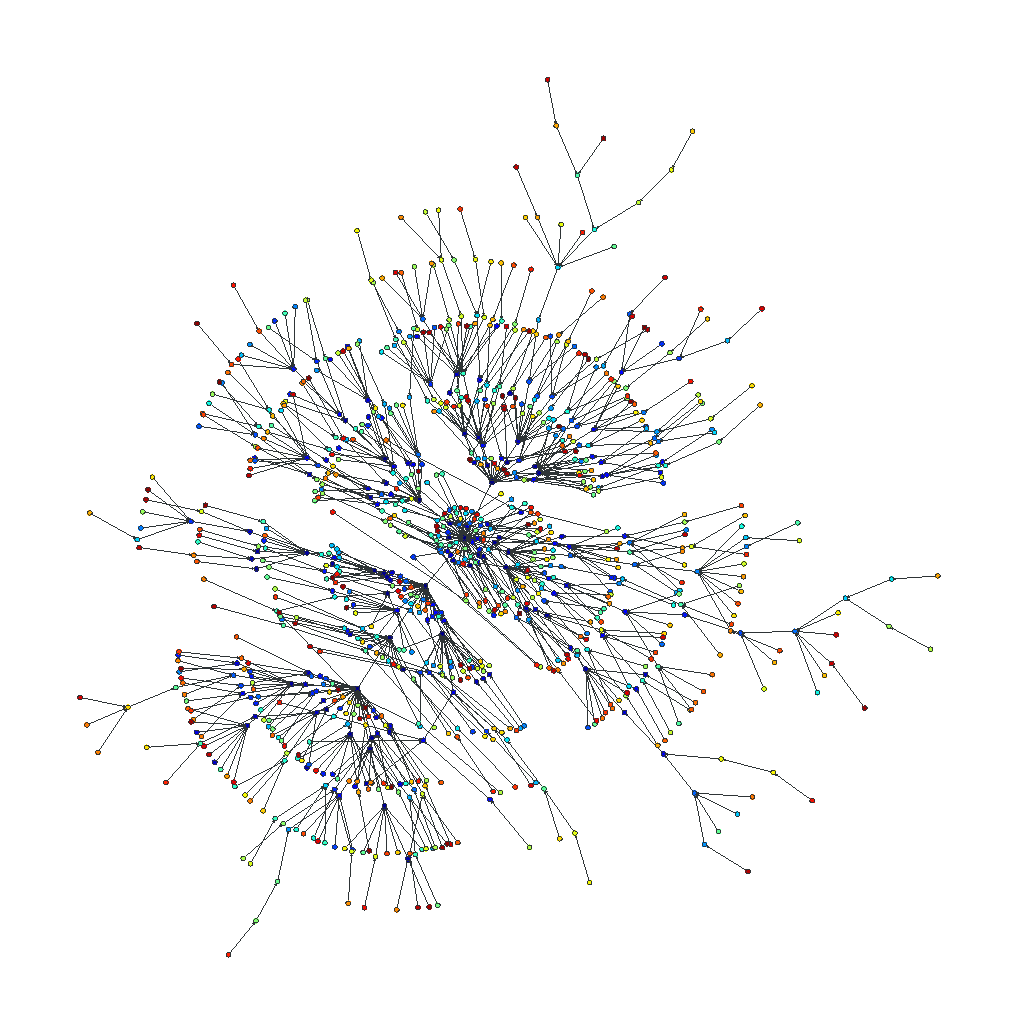
\includegraphics[width=0.4\textwidth]{../graphs/scale-free1000.pdf}
  }
  \hspace{1em}
  \subfloat[N = 10000]{
    \label{fig:scale-free-graph10000}
    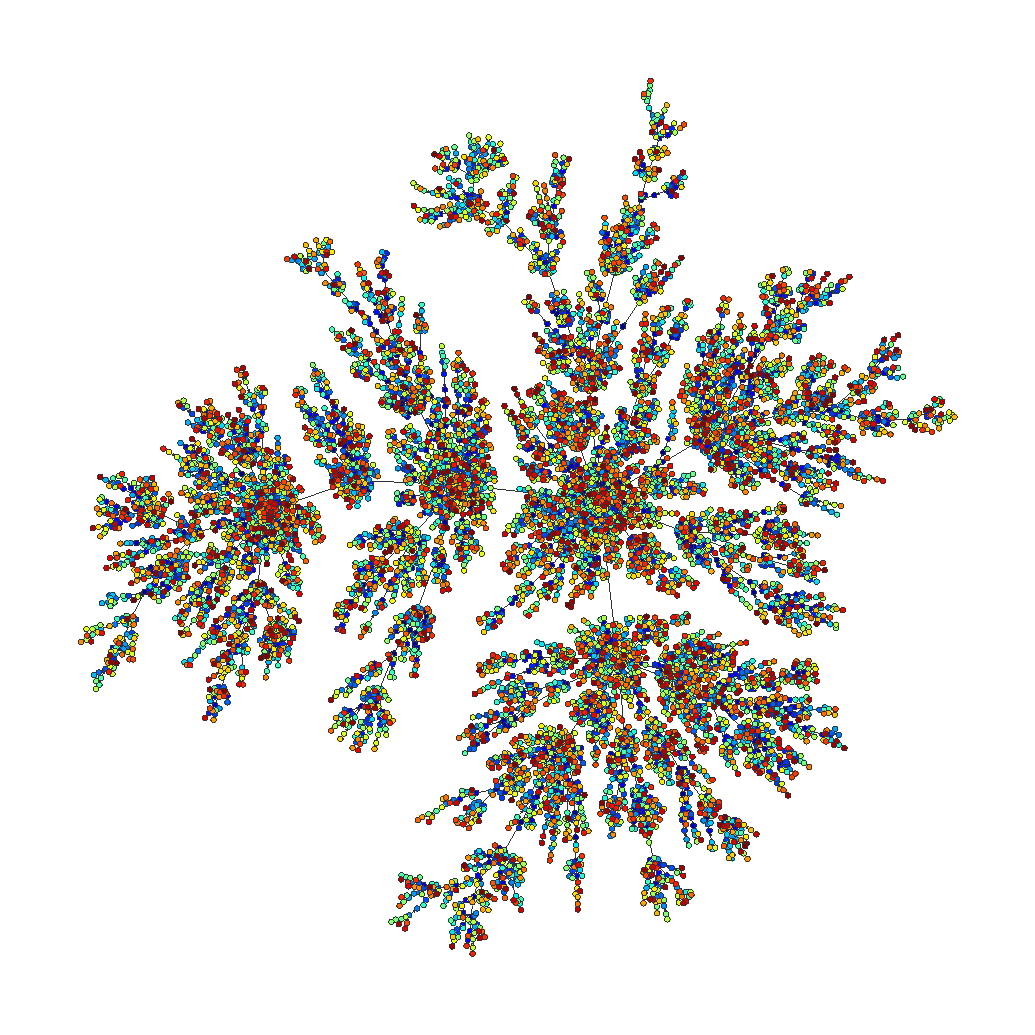
\includegraphics[width=0.4\textwidth]{../graphs/scale-free10000.pdf}
  }
  \hspace{1em}
  \caption{Scale-free networks with N nodes}
  \label{fig:scale-free-graphs}
\end{figure}

\newpage
\subsubsection{Plots}
Here we give the graphs plotting the total degree of the graphs that uses
the Barabasi algoritm above.\\
\begin{figure}[H]
  \centering
  \subfloat[N = 10]{
    \label{fig:scale-free-hist10}
    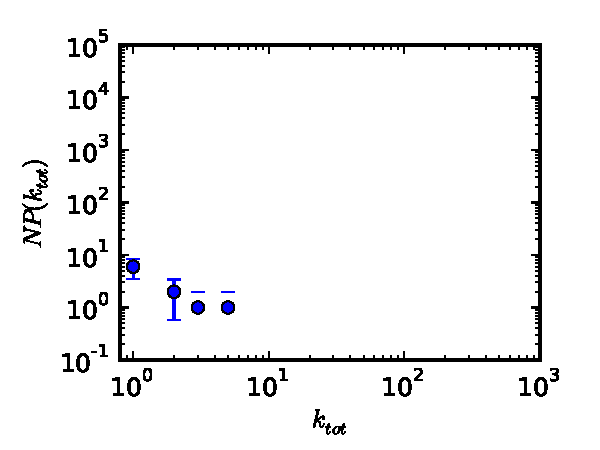
\includegraphics[width=0.4\textwidth]{../hist/scale-free10.pdf}
  }
  \hspace{1em}
  \subfloat[N = 100]{
    \label{fig:scale-free-hist100}
    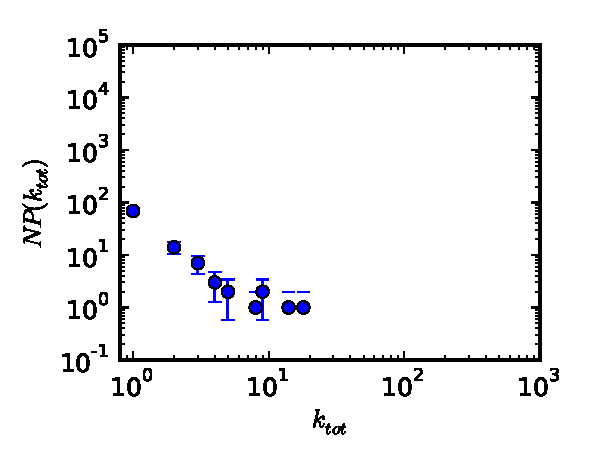
\includegraphics[width=0.4\textwidth]{../hist/scale-free100.pdf}
  }
  \hspace{1em}
  \subfloat[N = 1000]{
    \label{fig:scale-free-hist1000}
    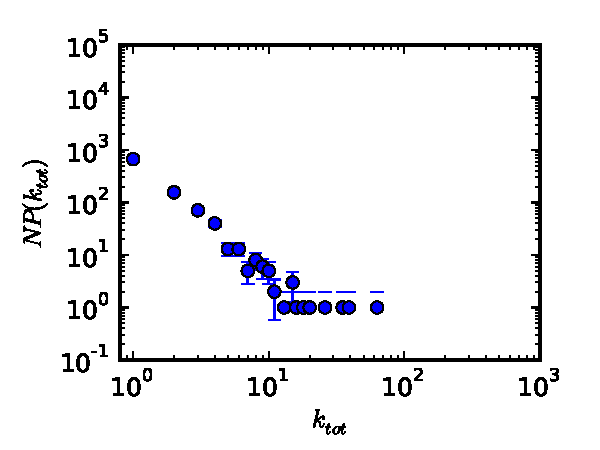
\includegraphics[width=0.4\textwidth]{../hist/scale-free1000.pdf}
  }
  \hspace{1em}
  \subfloat[N = 10000]{
    \label{fig:scale-free-hist10000}
    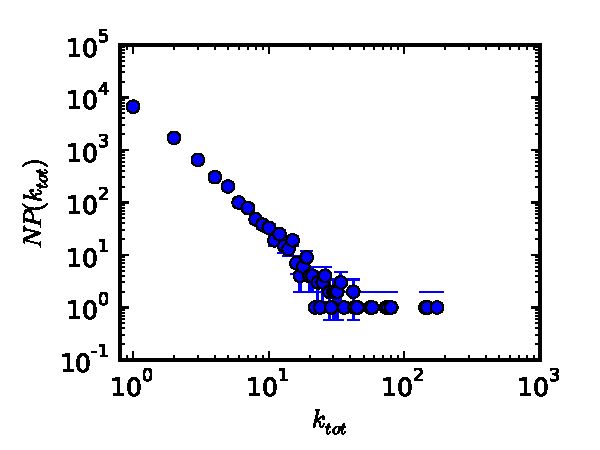
\includegraphics[width=0.4\textwidth]{../hist/scale-free10000.pdf}
  }
  \hspace{1em}
  \caption{Total-degree histogram of scale-free networks with N nodes}
  \label{fig:scale-free-histograms}
\end{figure}

\newpage
\subsection{SIR}
A SIR is a model to simulate the way a disease spreads through some population. SIR stands for Susceptible, Infected, Recovered/resistant. These are the states each member of the population can be in. In our implementation we have added a fourth state: Dead. 
We have implemented a very basic version of the SIR, to run on our generated networks. 
All the nodes are initialised as Susceptible. Then a small number of nodes
are infected, and possibly some nodes are marked as resistant. Then we move
on to simulate contacts. In each step a couple of things happen:\\

\begin{itemize}
  \item All the Susceptible nodes can be infected by an Infected neighbour. An Infected node infects a Susceptible node with chance Pinf.
  \item All the infected nodes can die with probability Pdeath or recover and become resistant with probability Precover. 
  \item The dead and recovered nodes don't change state anymore.
\end{itemize}

The simulation will take N steps. 

\newpage
\section{Measurements}
Here is where we present our measurements on both implementations of a
small-world network.\\
\subsection{Watts-Strogatz compared to Barabasi}
Here we give out analysis from comparing Watts-Strogatz networks with
Barabasi networks from different sizes.\\

\scalebox{0.7}{
  \begin{tabular}{c c | c | c | c | c | c |}
    \cline{3-7}
    & & \multicolumn{4}{c}{Watts-Strogatz} &
    \multicolumn{1}{|c|}{\multirow{2}{*}{Barabasi}} \\
    \cline{1-6}
    \multicolumn{1}{|c|}{Nodes} & Variables & K = 2, b = 0.05 & K = 2, b = 0.2 & K = 4, b =
    0.05 & K = 4, b = 0.2 & \\ 
    \hline

    \multicolumn{1}{|c|}{\multirow{4}{*}{N = 10}} & Clustering & 0.338 &
    0.435 & 0.8648 &  & 0.0\\ \cline{2-7}
    \multicolumn{1}{|c|}{} & Diameter & 3 & 3 & 2 & & 4\\ \cline{2-7}
    \multicolumn{1}{|c|}{} & Average degree & 4.0 & 4.0 & 8.0 & & 1.8\\ \cline{2-7}
    \multicolumn{1}{|c|}{} & Maximal degree & 5 & 5 & 9 & & 5\\ \cline{2-7}
    \hline

    \multicolumn{1}{|c|}{\multirow{4}{*}{N = 20}} & Clustering & 0.390 & 0.330 &  
    0.5628 & 0.479 & 0.0\\ \cline{2-7}
    \multicolumn{1}{|c|}{} & Diameter & 5 & 4 & 3 & 3 & 5\\ \cline{2-7}
    \multicolumn{1}{|c|}{} & Average degree & 4.0 & 4.0 & 8.0 & 8.0 & 1.9\\ \cline{2-7}
    \multicolumn{1}{|c|}{} & Maximal degree & 5 & 5 & 9 & 10 & 6\\ \cline{2-7}
    \hline

    \multicolumn{1}{|c|}{\multirow{4}{*}{N = 30}} & Clustering & 0.4098 & 0.3315 & 
    0.5229 & 0.3658 & 0.0\\ \cline{2-7}
    \multicolumn{1}{|c|}{} & Diameter & 7 & 7 & 4 & 3 & 6\\ \cline{2-7}
    \multicolumn{1}{|c|}{} & Average degree & 4.0 & 4.0 & 8.0 & 8.0 & 1.9333\\
    \cline{2-7}
    \multicolumn{1}{|c|}{} & Maximal degree & 5 & 6 & 10 & 11 & 9\\ \cline{2-7}
    \hline

    \multicolumn{1}{|c|}{\multirow{4}{*}{N = 40}} & Clustering & 0.4462 & 0.238
    & 0.5759 & 0.3181 & 0.0\\ \cline{2-7}
    \multicolumn{1}{|c|}{} & Diameter & 10 & 5 & 5 & 4 & 7 \\ \cline{2-7}
    \multicolumn{1}{|c|}{} & Average degree & 4.0 & 4.0 & 8.0 & 8.0 & 1.95\\ \cline{2-7}
    \multicolumn{1}{|c|}{} & Maximal degree & 5 & 6 & 9 & 10 & 10\\ \cline{2-7}
    \hline

    \multicolumn{1}{|c|}{\multirow{4}{*}{N = 50}} & Clustering & 0.3689 & 0.2866
    & 0.5501 & 0.3416 & 0.0\\ \cline{2-7}
    \multicolumn{1}{|c|}{} & Diameter & 8 & 6 & 5 & 4 & 7 \\ \cline{2-7}
    \multicolumn{1}{|c|}{} & Average degree & 4.0 & 4.0 & 8.0 & 8.0 & 1.96\\ \cline{2-7}
    \multicolumn{1}{|c|}{} & Maximal degree & 5 & 6 & 9 & 12 & 13\\ \cline{2-7}
    \hline

    \multicolumn{1}{|c|}{\multirow{4}{*}{N = 100}} & Clustering & 0.4547 & 0.2736 
    & 0.5655 & 0.3508 & 0.0\\ \cline{2-7}
    \multicolumn{1}{|c|}{} & Diameter & 15 & 8 & 6 & 5 & 7\\ \cline{2-7}
    \multicolumn{1}{|c|}{} & Average degree & 4.0 & 4.0 & 8.0 & 8.0 & 1.98\\ \cline{2-7}
    \multicolumn{1}{|c|}{} & Maximal degree & 5 & 6 & 9 & 11 & 18\\ \cline{2-7}
    \hline

    \multicolumn{1}{|c|}{\multirow{4}{*}{N = 1000}} & Clustering & 0.4254 & 0.2502
    & 0.5410 & 0.3185 & 0.0\\ \cline{2-7}
    \multicolumn{1}{|c|}{} & Diameter & 30 & 13 & 10 & 7 & 10 \\ \cline{2-7}
    \multicolumn{1}{|c|}{} & Average degree & 4.0 & 4.0 & 8.0 & 8.0 & 1.998\\
    \cline{2-7}
    \multicolumn{1}{|c|}{} & Maximal degree & 6 & 7 & 11 & 12 & 63\\ \cline{2-7}
    \hline

    \multicolumn{1}{|c|}{\multirow{4}{*}{N = 10000}} & Clustering & 0.4235 & 0.2466
    & 0.5467 & 0.3257 & 0.0\\ \cline{2-7}
    \multicolumn{1}{|c|}{} & Diameter & 39 & 18 & 15 & 9 & 16 \\ \cline{2-7}
    \multicolumn{1}{|c|}{} & Average degree & 4.0 & 4.0 & 8.0 & 8.0 & 1.9998\\
    \cline{2-7}
    \multicolumn{1}{|c|}{} & Maximal degree & 7 & 9 & 12 & 14 & 174\\ \cline{2-7}
    \hline

  \end{tabular}
}

\subsection{Watts-Strogatz plots}
Here are some plots taken from the Watts-Strogatz algorithms with different
parameters for the \texttt{N}, \texttt{K} and \texttt{b}.\\

\begin{figure}[H]
  \centering
  \subfloat[N = 30, K = 4, b = 0.05]{
    \label{fig:watts-30-4-0.05}
    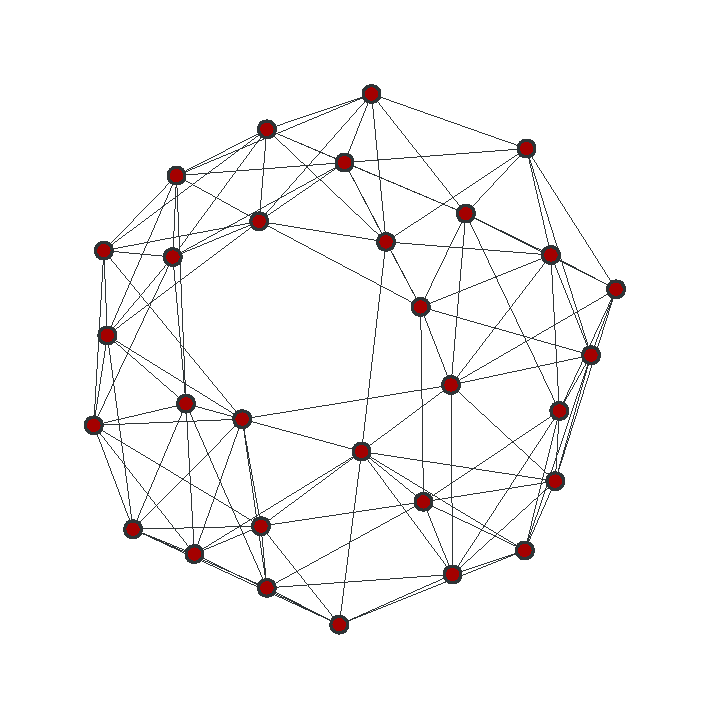
\includegraphics[width=0.6\textwidth]{../graphs/watts-30-4-005.pdf}
  }
  \hspace{1em}
  \subfloat[N = 30, K = 4, b = 0.2]{
    \label{fig:watts-30-4-0.2}
    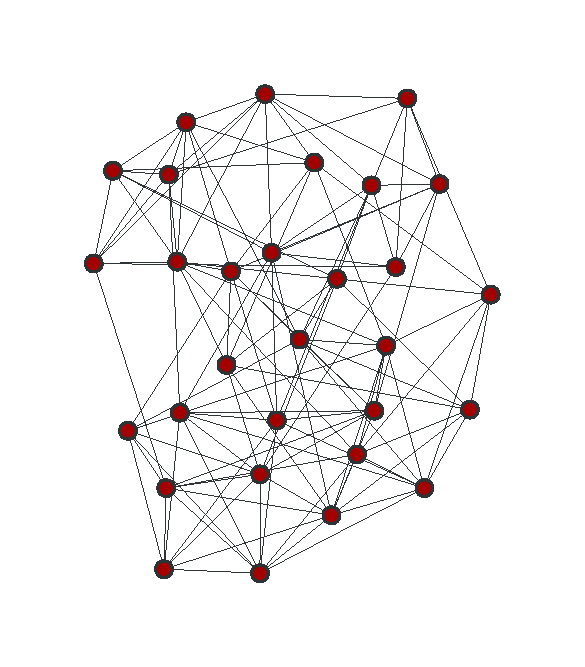
\includegraphics[width=0.6\textwidth]{../graphs/watts-30-4-02.pdf}
  }
  \hspace{1em}
  \caption{Watts-Strogatz network with \texttt{N} nodes, mean degree of the
  nodes \texttt{K} and propabilty of rewiring \texttt{b}}
  \label{fig:watts-strogatz-networks}
\end{figure}

As you can see the higher the value of \texttt{b} is, the more irregular the
network becomes.

\newpage

\subsection{SIR Plots}
\begin{figure}[H]
  \centering
  \subfloat[Step 1]{
    \label{fig:1SIR}
    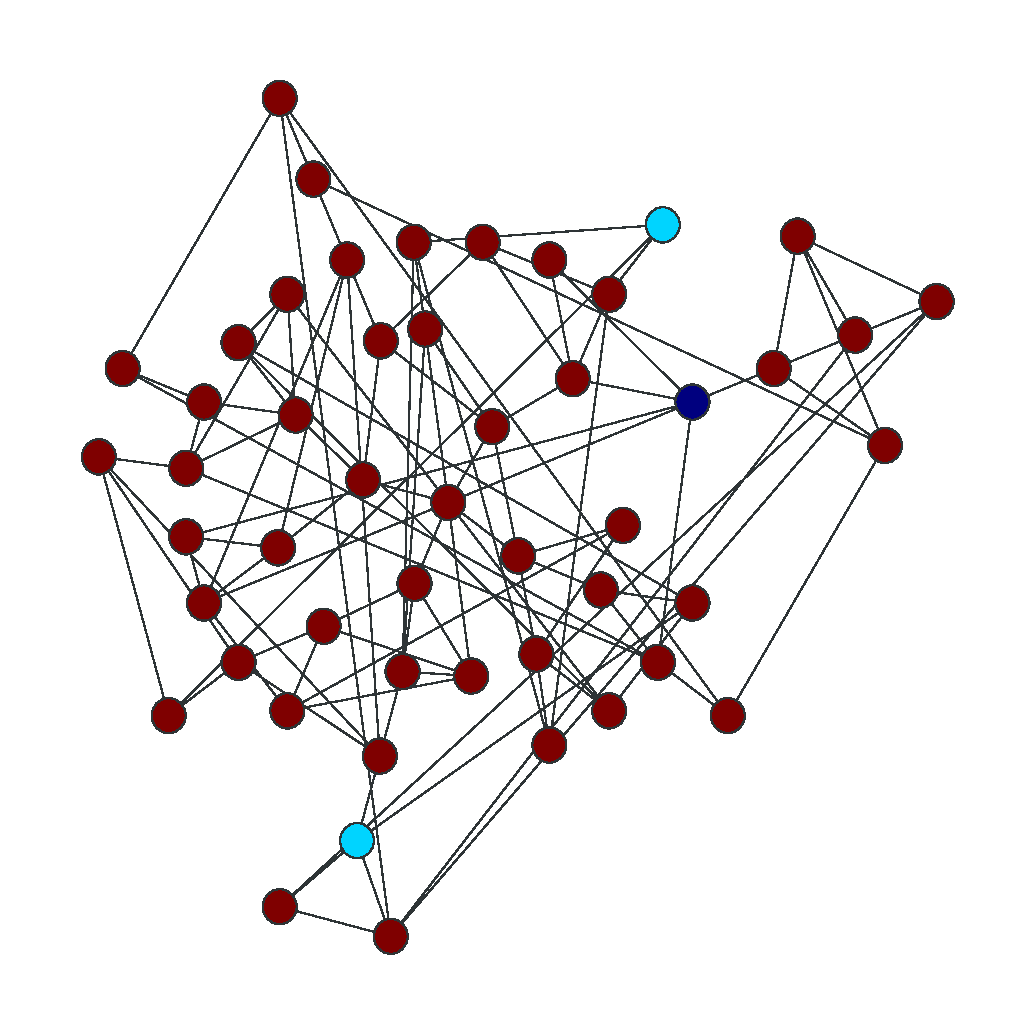
\includegraphics[width=0.4\textwidth]{../graphs/0SIR.pdf}
  }
  \hspace{1em}
  \subfloat[Step 2]{
    \label{fig:2SIR}
    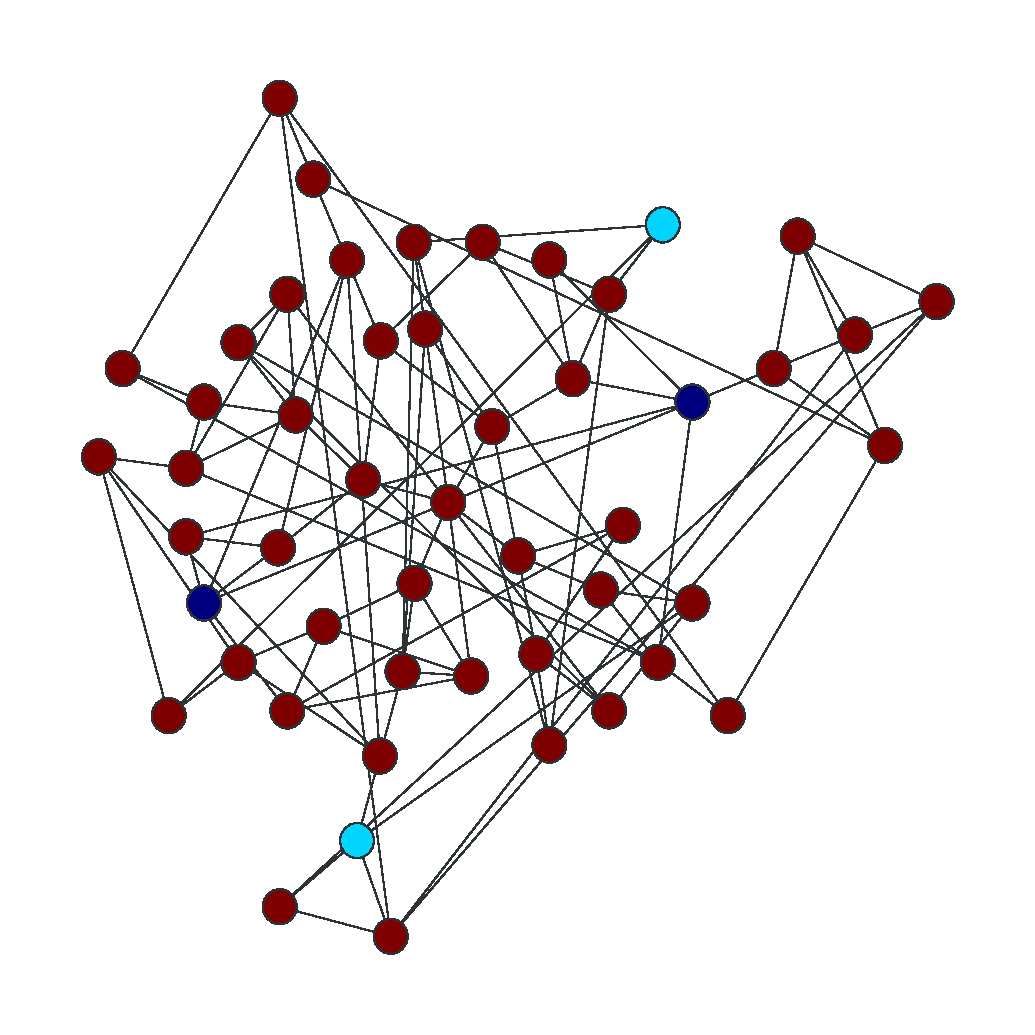
\includegraphics[width=0.4\textwidth]{../graphs/1SIR.pdf}
  }
  \hspace{1em}
  \subfloat[Step 3]{
    \label{fig:3SIR}
    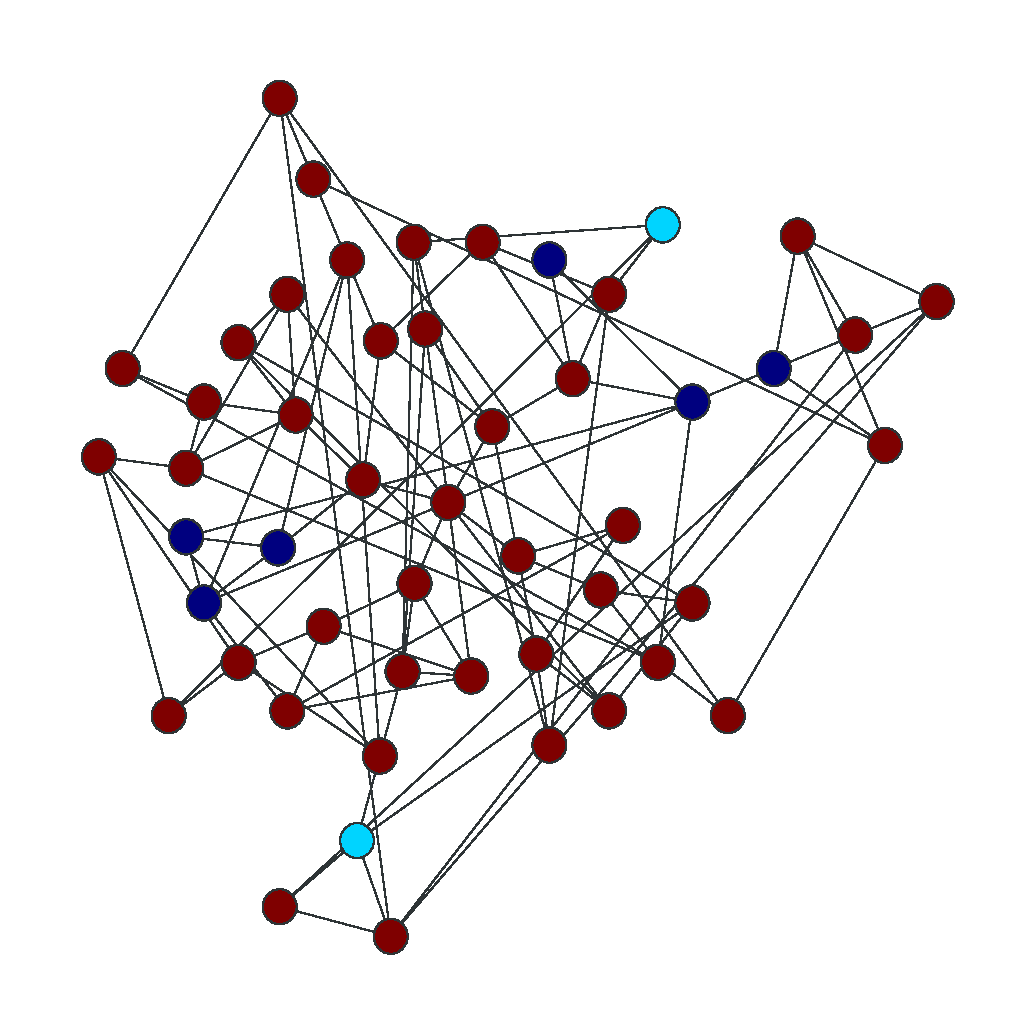
\includegraphics[width=0.4\textwidth]{../graphs/2SIR.pdf}
  }
  \hspace{1em}
  \subfloat[Step 4]{
    \label{fig:4SIR}
    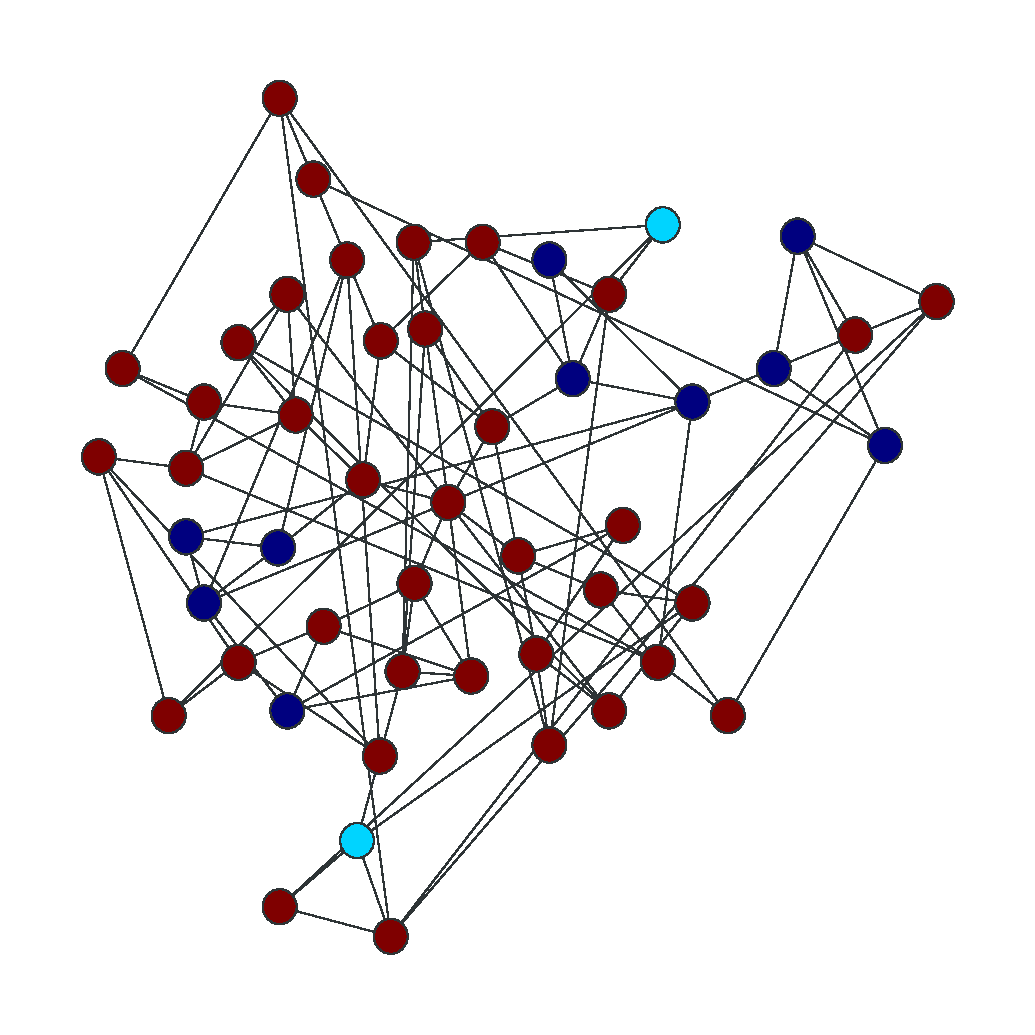
\includegraphics[width=0.4\textwidth]{../graphs/3SIR.pdf}
  }
  \hspace{1em}
  \caption{Progress of a SIR-model infection in a Watts-Strogatz network}
  \label{fig:SIR1-4}
\end{figure}

\newpage
\begin{figure}[H]
  \centering
  \subfloat[Step 5]{
    \label{fig:5SIR}
    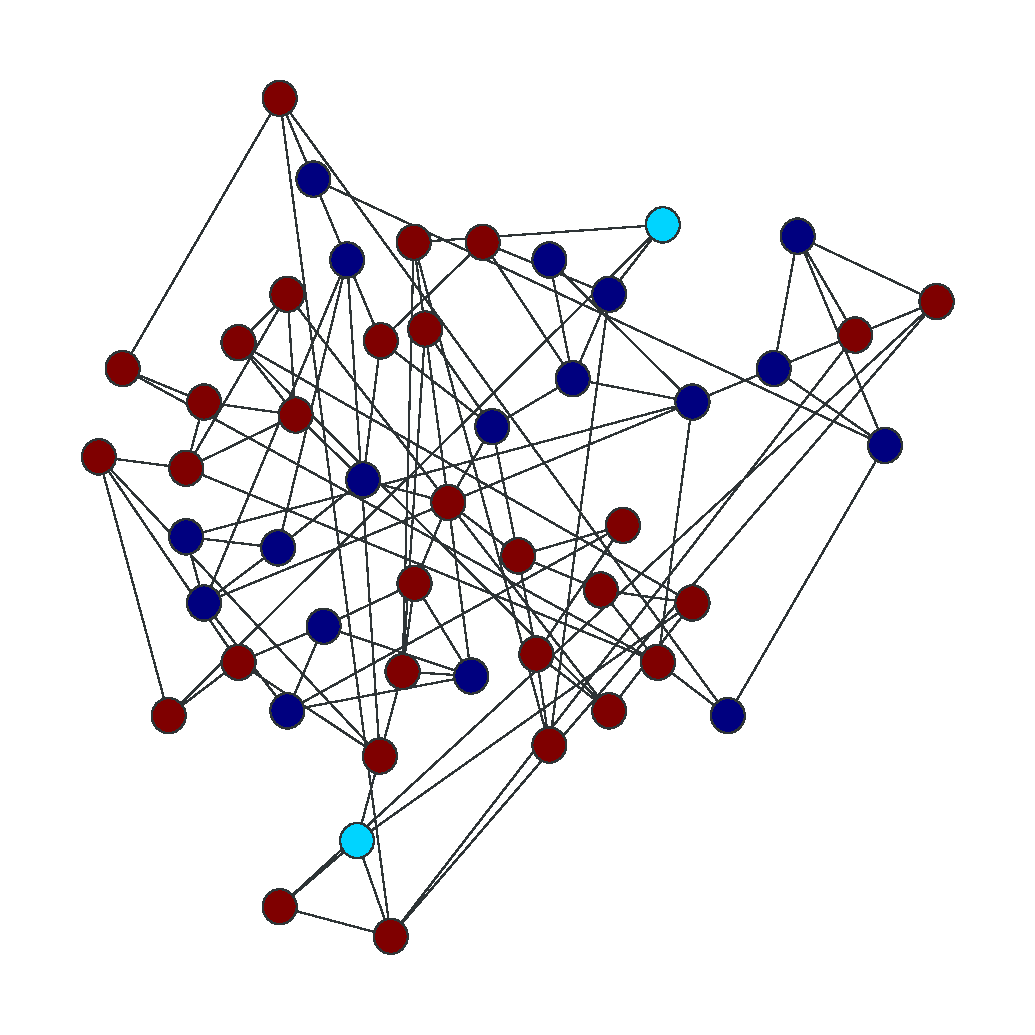
\includegraphics[width=0.4\textwidth]{../graphs/4SIR.pdf}
  }
  \hspace{1em}
  \subfloat[Step 6]{
    \label{fig:6SIR}
    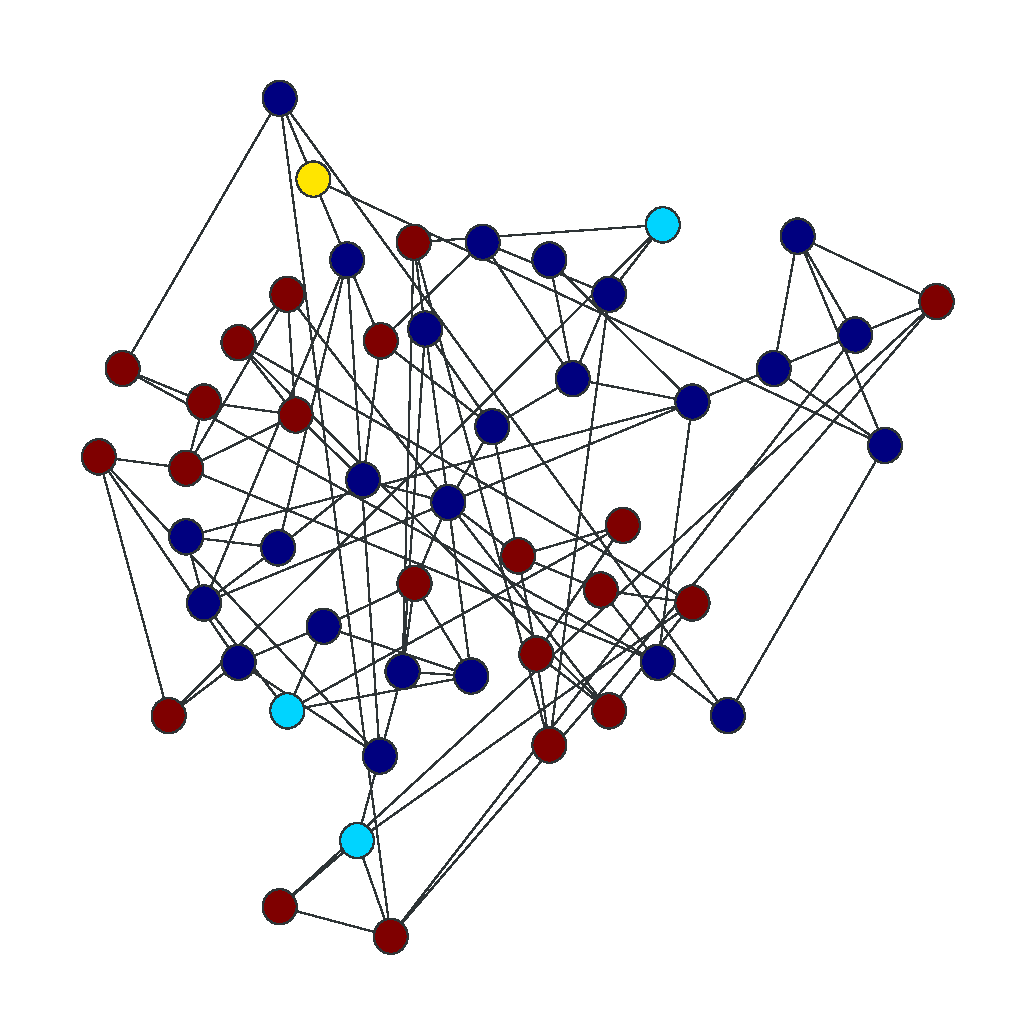
\includegraphics[width=0.4\textwidth]{../graphs/5SIR.pdf}
  }
  \hspace{1em}
  \subfloat[Step 7]{
    \label{fig:7SIR}
    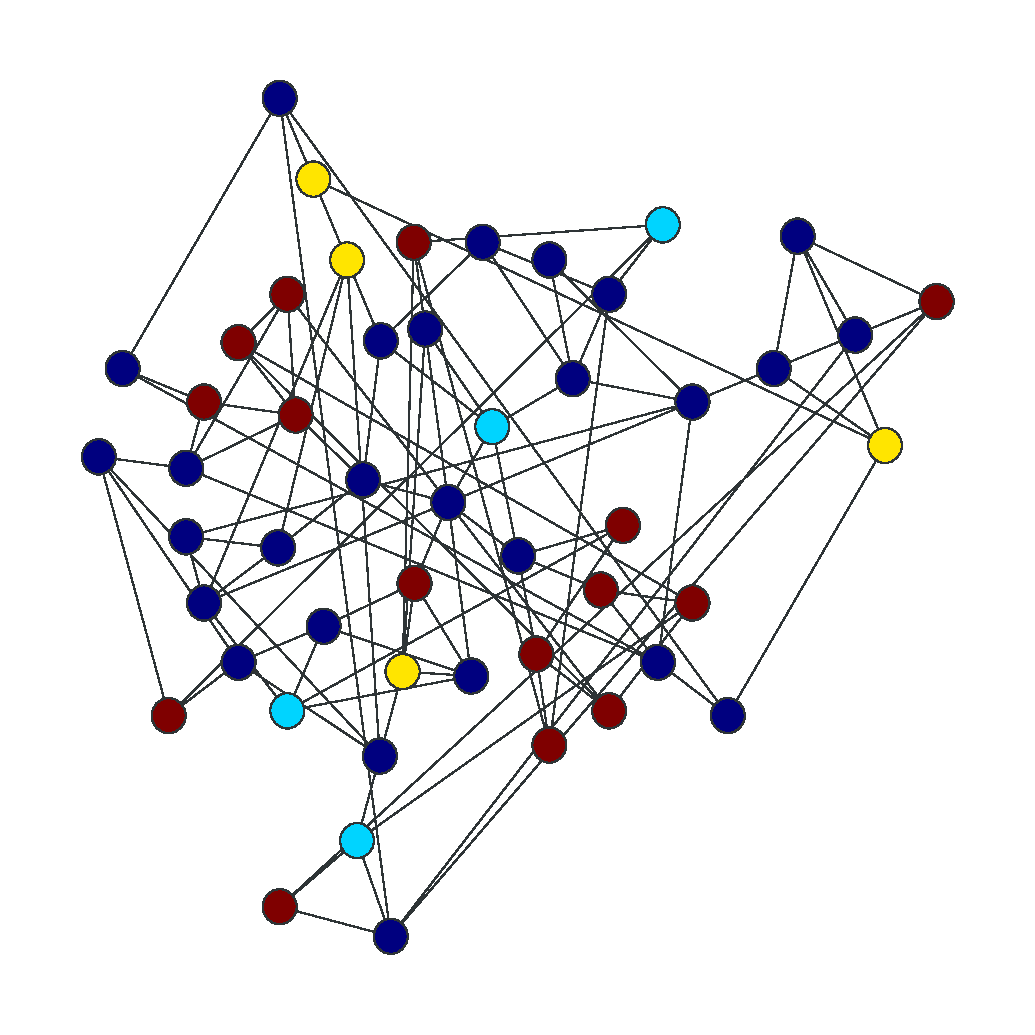
\includegraphics[width=0.4\textwidth]{../graphs/6SIR.pdf}
  }
  \hspace{1em}
  \subfloat[Step 8]{
    \label{fig:8SIR}
    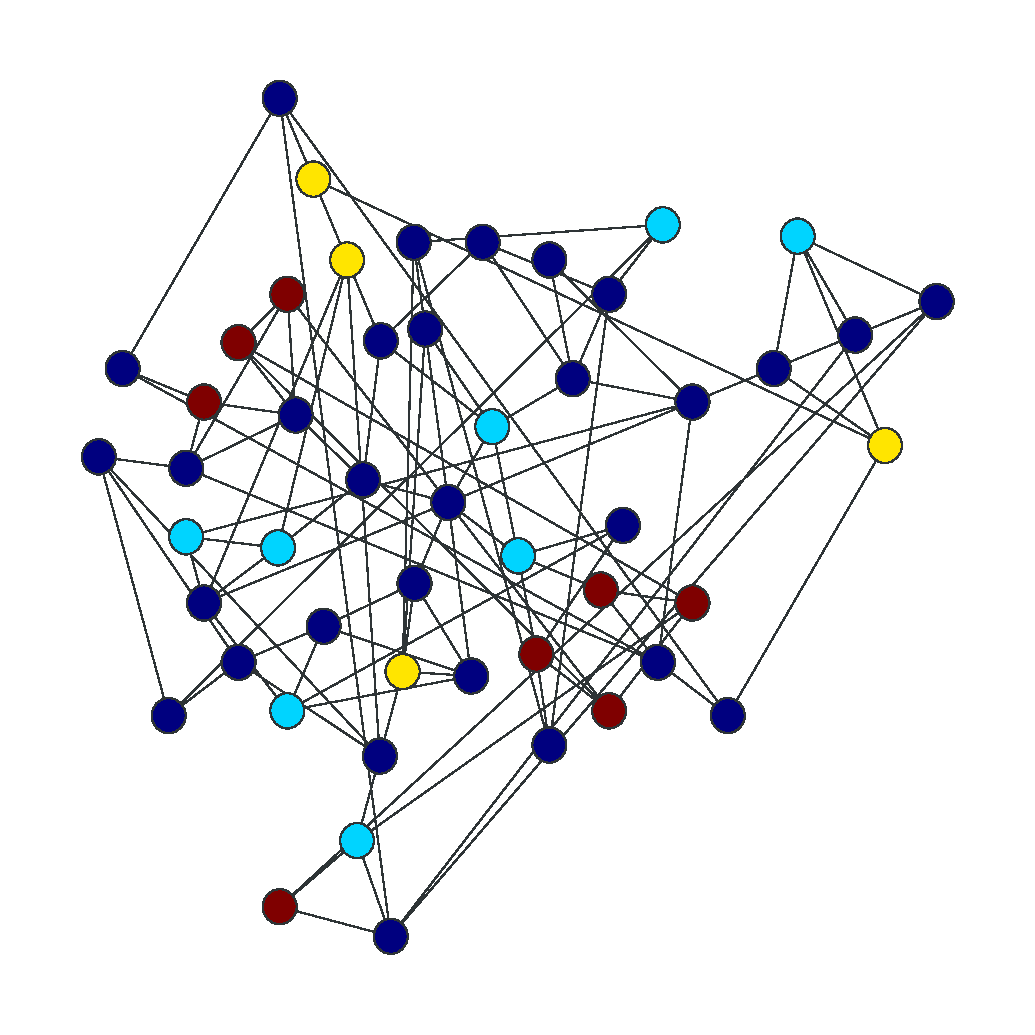
\includegraphics[width=0.4\textwidth]{../graphs/7SIR.pdf}
  }
  \hspace{1em}
  \caption{Progress of a SIR-model infection in a Watts-Strogatz network}
  \label{fig:SIR5-8}
\end{figure}

\newpage
\subsection{Analysis SIR}
After running the model on a network created by the Watts-Strogatz algorithm we can see that the random nature of the network allows it to spread to other parts of the network quite quickly. Also if we include a number of resistant nodes it will not have a huge effect on the spread rate. Sure the resistant nodes will block the infection, but because there are so many connections the infection will eventually get there via another route. 
In the Barabasi generated networks show a very different behaviour. Because
the tree-like structure of the tree, there are a couple of hubs in the
network who determine whether the infection will spread rapidly. If a hub is
infected, the infection spreads very rapidly to all of the nodes connected
to the hub. If, on the other hand, the hub is resistant, the infection will
be blocked, and all the other parts of the network behind the hub will be
safe. Because of the random factor in infection and resistance, it is almost
impossible to predict how far an infection will reach. It could reach a big
hub and spread through the whole network, or it could encounter a resistant
node on the first step and not carry any further.\\

In general the infections in the Watts-Strogatz model will carry further, but this will take longer then in the Barabasi network. In Barabasi the infection will often be contained to a part of the network, but the infection will spread quickly. 
This can be explained by the high number of connections but the low maximum degree in the Watts-Strogatz. There are a lot of ways to infect parts of the network and it will spread steadily. The high maximum degree and the low number of connections explain the Barabasi behaviour. Once a hub is infected, it will spread extremely fast but once a route to a part of the network is blocked by a resistant node, there is no other way for the infection to get there.

\newpage
\appendix

\end{document}


